% Figura: fluxograma do ILS-VND
\documentclass[tikz,border=4pt]{standalone}
\usepackage[utf8]{inputenc}
\usepackage[T1]{fontenc}
\usepackage{helvet}
\renewcommand{\familydefault}{\sfdefault}
\usepackage{amsmath}
\usepackage[eulergreek]{sansmath}
\sansmath
\usetikzlibrary{shapes.geometric,arrows.meta,positioning,fit,backgrounds,calc}
\tikzset{
  etapa/.style={draw=blue!60!black, rounded corners=4pt, fill=blue!4, inner sep=8pt},
  bloco/.style={draw=black!70, rounded corners=2pt, fill=white, align=center,
                font=\small, minimum height=1.1cm, text width=2.9cm},
  decisao/.style={diamond, draw=black!70, fill=yellow!15, aspect=1.8, align=center,
                  font=\small, inner sep=1pt},
  fim/.style={draw=black!70, rounded corners=8pt, fill=green!12, align=center,
              font=\small, minimum height=1.0cm, text width=3.1cm},
  falha/.style={draw=red!60!black, rounded corners=8pt, fill=red!8, align=center,
                font=\small, minimum height=0.8cm},
  seta/.style={-{Stealth[length=2.2mm]}, line width=0.7pt},
  rotetapa/.style={font=\small\bfseries, text=blue!60!black, anchor=south west},
}
\begin{document}
\hyphenpenalty=10000\exhyphenpenalty=10000
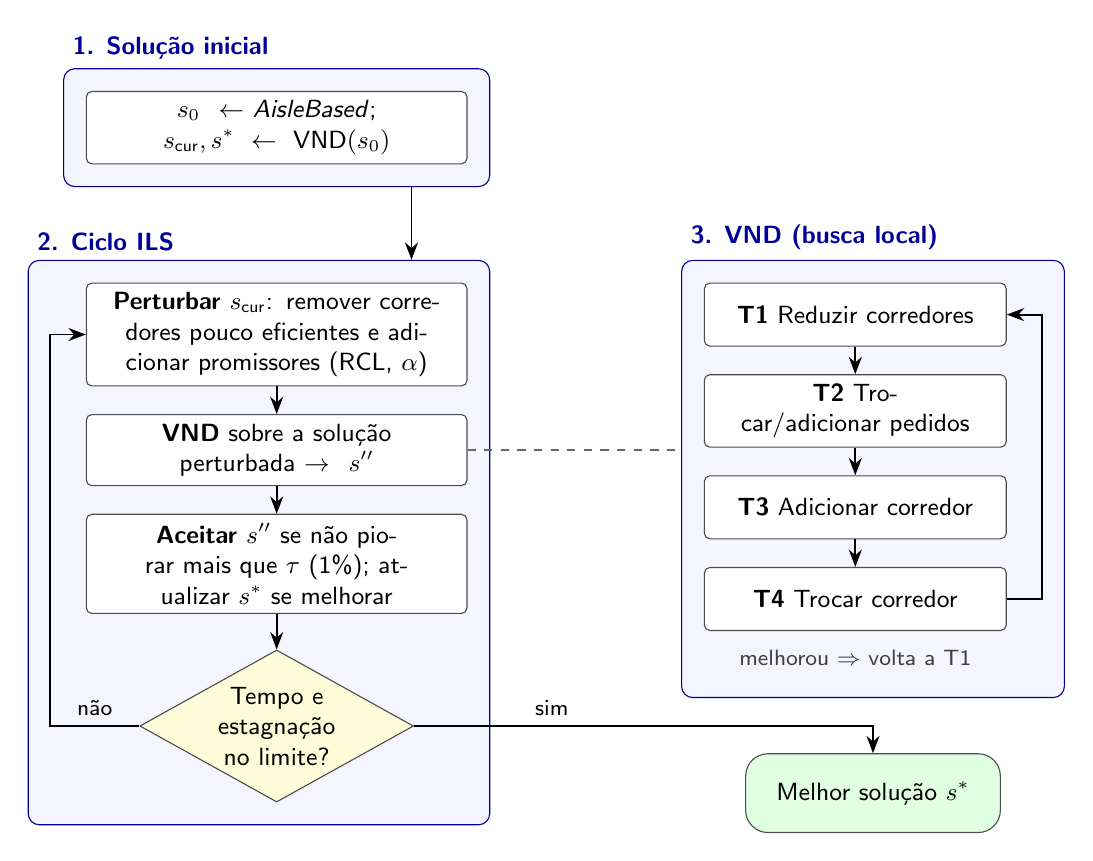
\begin{tikzpicture}[node distance=0.35cm]
\tikzset{pq/.style={bloco, minimum height=0.9cm},
         tier/.style={bloco, minimum height=0.8cm, text width=3.6cm, fill=white}}

% ---------- 2. Ciclo ILS (definido primeiro para alinhar) ----------
\node[pq, text width=4.6cm] (pert) {\textbf{Perturbar} $s_{\text{cur}}$: remover corredores pouco eficientes e adicionar promissores (RCL, $\alpha$)};
\node[pq, below=of pert, text width=4.6cm] (vnd) {\textbf{VND} sobre a solução perturbada $\to s''$};
\node[pq, below=of vnd, text width=4.6cm] (acc) {\textbf{Aceitar} $s''$ se não piorar mais que $\tau$ (1\%); atualizar $s^\ast$ se melhorar};
\node[decisao, below=0.45cm of acc] (cont) {Tempo e\\estagnação\\no limite?};
\coordinate (lp) at ($(pert.west)+(-0.45,0)$);
\begin{scope}[on background layer]
  \node[etapa, fit=(pert)(vnd)(acc)(cont)(lp)] (e2) {};
\end{scope}
\node[rotetapa] at (e2.north west) {2. Ciclo ILS};
\draw[seta] (pert) -- (vnd);
\draw[seta] (vnd) -- (acc);
\draw[seta] (acc) -- (cont);
\draw[seta] (cont.west) -- node[above, font=\footnotesize] {não} (cont.west -| lp) -- (lp) -- (pert.west);

% ---------- 1. Solução inicial ----------
\node[pq, above=1.5cm of pert, text width=4.6cm] (ini) {$s_0 \gets$ \textit{AisleBased};\quad $s_{\text{cur}}, s^\ast \gets \text{VND}(s_0)$};
\begin{scope}[on background layer]
  \node[etapa, fit=(ini)] (e1) {};
\end{scope}
\node[rotetapa] at (e1.north west) {1. Solução inicial};
\draw[seta] ([xshift=-1.0cm]e1.south east) -- ([xshift=-1.0cm]e1.south east |- e2.north);

% ---------- 3. VND: tiers de vizinhança ----------
\node[tier, right=3.0cm of pert.north east, anchor=north west] (t1) {\textbf{T1} Reduzir corredores};
\node[tier, below=of t1] (t2) {\textbf{T2} Trocar/adicionar pedidos};
\node[tier, below=of t2] (t3) {\textbf{T3} Adicionar corredor};
\node[tier, below=of t3] (t4) {\textbf{T4} Trocar corredor};
\coordinate (rp) at ($(t1.east)+(0.45,0)$);
\node[font=\footnotesize, below=0.12cm of t4, text=black!75] (nota) {melhorou $\Rightarrow$ volta a T1};
\begin{scope}[on background layer]
  \node[etapa, fit=(t1)(t2)(t3)(t4)(rp)(nota)] (e3) {};
\end{scope}
\node[rotetapa] at (e3.north west) {3. VND (busca local)};
\draw[seta] (t1) -- (t2);
\draw[seta] (t2) -- (t3);
\draw[seta] (t3) -- (t4);
\draw[seta] (t4.east) -- (t4.east -| rp) -- node[right, font=\footnotesize, align=left, pos=0.5] {} (rp) -- (t1.east);

% ligação VND (ciclo) -> detalhe
\draw[dashed, black!60, line width=0.6pt] (vnd.east) -- (vnd.east -| e3.west);

% ---------- resultado ----------
\node[fim, below=0.7cm of e3, text width=3.0cm] (res) {Melhor solução $s^\ast$};
\draw[seta] (cont.east) -- node[above, font=\footnotesize, pos=0.3] {sim} (cont.east -| res.north) -- (res.north);

\end{tikzpicture}
\end{document}
